% !TEX TS-program = pdflatex
% !TEX encoding = UTF-8 Unicode

% This is a simple template for a LaTeX document using the "article" class.
% See "book", "report", "letter" for other types of document.

\documentclass[11pt]{article} % use larger type; default would be 10pt
\usepackage{natbib}
\usepackage{mathtools}
\usepackage{graphicx}


\usepackage[utf8]{inputenc} % set input encoding (not needed with XeLaTeX)


%%% Examples of Article customizations
% These packages are optional, depending whether you want the features they provide.
% See the LaTeX Companion or other references for full information.

%%% PAGE DIMENSIONS
\usepackage{geometry} % to change the page dimensions
\geometry{a4paper} % or letterpaper (US) or a5paper or....
% \geometry{margin=2in} % for example, change the margins to 2 inches all round
% \geometry{landscape} % set up the page for landscape
%   read geometry.pdf for detailed page layout information

\usepackage{graphicx} % support the \includegraphics command and options

% \usepackage[parfill]{parskip} % Activate to begin paragraphs with an empty line rather than an indent

%%% PACKAGES
\usepackage{booktabs} % for much better looking tables
\usepackage{array} % for better arrays (eg matrices) in maths
\usepackage{paralist} % very flexible & customisable lists (eg. enumerate/itemize, etc.)
\usepackage{verbatim} % adds environment for commenting out blocks of text & for better verbatim
\usepackage{subfig} % make it possible to include more than one captioned figure/table in a single float
% These packages are all incorporated in the memoir class to one degree or another...

%%% HEADERS & FOOTERS
\usepackage{fancyhdr} % This should be set AFTER setting up the page geometry
\pagestyle{fancy} % options: empty , plain , fancy
\renewcommand{\headrulewidth}{0pt} % customise the layout...
\lhead{}\chead{}\rhead{}
\lfoot{}\cfoot{\thepage}\rfoot{}

%%% SECTION TITLE APPEARANCE
\usepackage{sectsty}
\allsectionsfont{\sffamily\mdseries\upshape} % (See the fntguide.pdf for font help)
% (This matches ConTeXt defaults)

%%% ToC (table of contents) APPEARANCE
\usepackage[nottoc,notlof,notlot]{tocbibind} % Put the bibliography in the ToC
\usepackage[titles,subfigure]{tocloft} % Alter the style of the Table of Contents
\renewcommand{\cftsecfont}{\rmfamily\mdseries\upshape}
\renewcommand{\cftsecpagefont}{\rmfamily\mdseries\upshape} % No bold!

%%% END Article customizations


\title{Report \\ Automatic Polyphonic Piano Music Transcription}
\author{Agnieszka Szefer}
%\date{} % Activate to display a given date or no date (if empty),
         % otherwise the current date is printed 

\begin{document}

\newcommand{\myparagraph}[1]{\paragraph{#1}\mbox{}\\}
\maketitle

\tableofcontents

\section{Introduction}
Transcription of music is a very challenging task. Even after millions of years of evolution of our sense of hearing it is still difficult for a human without any prior musical education to tackle this problem. Only after long training some people may be able to transcribe music correctly. The problem of music transcription recenty gained interest of many researchers who proposed several solutions for automating this process. The ideas suggested work relatively fine for monophonic music, however in case of polyphonic music transcription, i.e. when at least two notes are played at the same time,  the results are still far from perfect.

\subsection{Motivation}
\subsection{Related Work}
\subsection{Objectives}
\subsection{Contributions}
\subsection{Report Outline}


\section{Problem Definition}

\subsection{Music Transcription}
The aim of this project is to automate the process of music transcription, i.e. generate a music notation representation of the given digital sound. I am going to work with piano music stored in Waveform Audio File Format (.wav). This format is uncompressed what ensures the highest quality of the recorded sound. Moreover, it is the most general music storage format and it can be easily converted to other popular formats such as .mp3 or .gsm. It is also easy to edit and manipulate with software. I chose piano music as pianos are capable of producing polyphonic sounds and this project focuses on the polyphonic pitch detection. Moreover, piano music is quite popular and the results of this project are therefore more likely to be used than in the case of less popular instrument music analysis. Finally, there exist a wide range of manually generated piano scores in a digital form that can be used in the evaluation phase of the project. 

The music notation I will generate is the modern five-line staff notation (see Figure ~\ref{fig:notes}). The notation uses notes on the staff to represent some features of the musical tones. A musical tone is characterised by its pitch, duration, loudness and timbre. We can identify the pitch of a tone from the location of a note on the staff. The duration is shown using different note values together with dots and ties. Loudness is expressed with annotations below the staff. Timbre is the quality of a sound and is specific to each instrument. Piano music notation includes two staffs, one for the right hand, starting with the treble clef, and one for the left hand, starting with the bass clef. The clef is followed by the key signature, specifying which notes will be flat or sharp throughout the piece, and the time signature of the piece.

\begin{figure}[h!]
\begin{center}
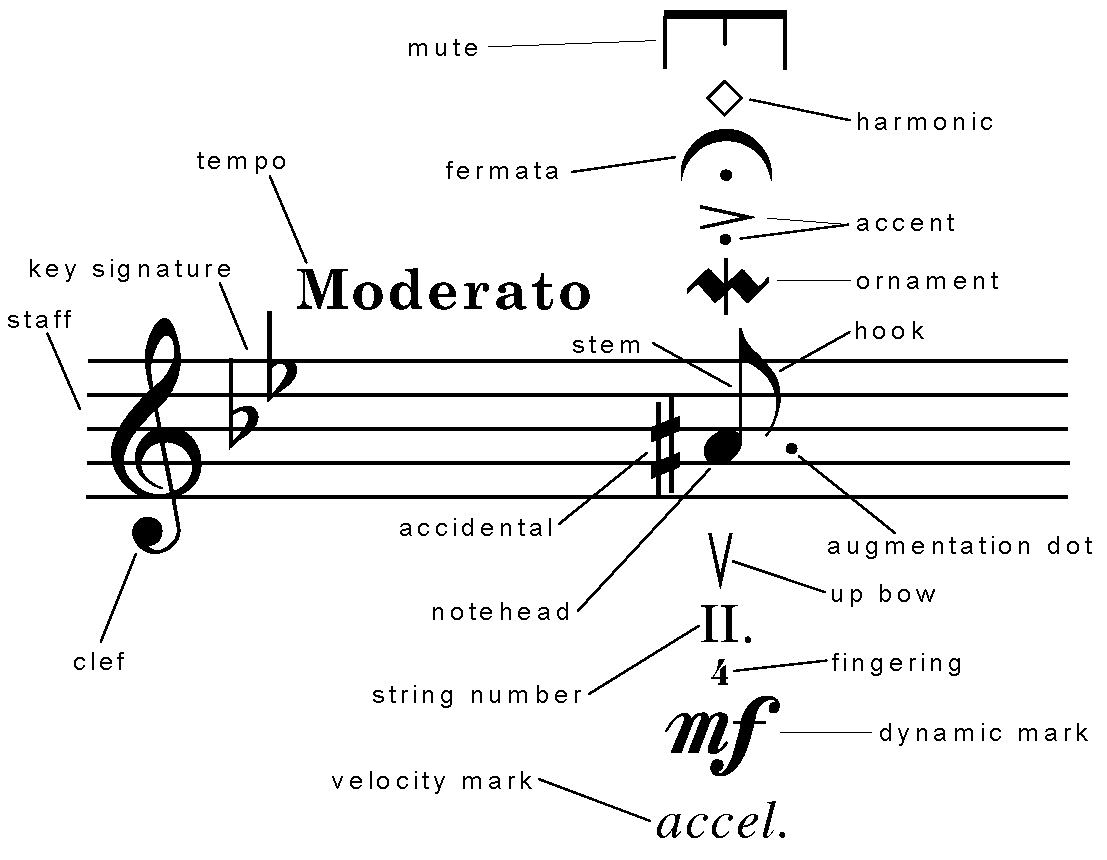
\includegraphics[scale=0.2]{note}
\end{center}
\caption{Description of music notation for the treble clef staff \citep*{notesWebsite}.}
\label{fig:notes}
\end{figure}

The notes are arranged on a quantised logarithmic scale, with 12 notes in each octave range. The fundamental frequency of a note \textit{n} can be calculated as 
\[440 Hz * 2^{n/12}  \]
where \textit{n} varies from -48 to 39 on a standard piano keyboard. The notes in each octave are lettered as C, C\#, D, D\#, E, F, ...  \citep*{Klapuri2006}.

\subsection{Onset Detection}
In order to detect the pitch we need to know in which part of the segment we should look for it. Therefore we need to know where the notes begin (where is their \textit{onset}), i.e. where their amplitude rises from zero to an initial peak. Some instruments may take up to 100ms or more to settle into a stable pitch \citep*{Roads1996}. Fortunately, pianos usually produce a loud attack of a note with a fast decay what makes the onset detection easier. I am going to use already developed onset detection methods to find the onsets and split the signal into onset frames. Onset detection methods are described in more detail in the further sections. 

\subsection{Pitch Detection}
After splitting the signal into onset frames we can concentrate on detecting the pitches of the notes in each segment. The sounds in each frame can appear as either single tones (\textit{monophonic signals}) or up to several concurrent tones (\textit{polyphonic signals}). The main difficulty is detecting the pitches of these simultaneously played tones. This project focuses on evaluating existing polyphonic pitch detection methods and finding ways how to improve them.

\subsection{Scores generation}
The final phase of the transcription is generating printable scores from the assembled discrete events, i.e. detected pitches and onsets. Taking into account the nature of the assembled data, the transcription will focus on correct placement of notes on the staff and identifying the key signature. However, less attention will be paid to the other characteristics of the notes, such as their duration or dynamics. As a possible extension, MIDI representation of the discrete events could be also generated. 

\section{Background}
This section introduces the concepts from musical theory and signal processing needed to understand the project. 


\subsection{Digital Sound Signal}
This section covers the basic concepts used in digital signal processing.

\subsubsection{Frequency}
Musical instruments or any other sources generate vibrations that are propagated through air or other medium in a form of a waveform. These vibrations are commonly known as \textit{sounds} and we are able to hear them because of the changes in the air pressure in our ears. If the pressure varies according to a repeating patterns we say that the sound has a \textit{periodic waveform} \citep*{Roads1996}.

One such pattern repetition is called a \textit{cycle}, and the \textit{fundamental frequency} is the number of cycles that occur per second. The frequency is measured in units of Hertz, where 1Hz means one cycle per second. The \textit{period} of a waveform is the lenght of the cycle and as it increases the frequency decreases.

\subsubsection{Time-domain Representation}
One way of representing a sound waveform is as a time-domain graph showing how the air pressure changes over time (see Figure ~\ref{fig:representations}). The \textit{amplitude} is the maximum displacement of the wave measured from its equilibrium position.

\subsubsection{Frequency-domain Representation}
A waveform may consist of not only the fundamental frequency, but also many other frequencies. The frequency-domain representation, also called the \textit{spectrum}, shows the frequencies that contribute to the sound (see Figure ~\ref{fig:representations}). Any frequency component is a \textit{partial}. A partial that is an integer multiple of the fundamental frequency is called a \textit{harmonic}.

\begin{figure}[h!]
\begin{center}
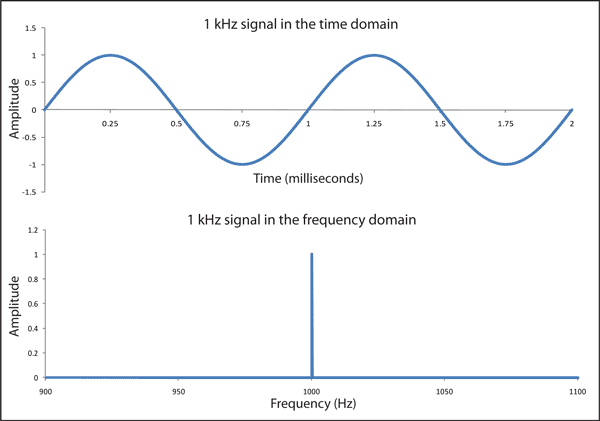
\includegraphics[scale=0.6]{TimeDomain}
\end{center}
\caption{Time-domain and frequency-domain representations.}
\label{fig:representations}
\end{figure}

\subsection{Pitch}
The subjective pitch is the height of a sound perceived by a listener. The fundamental frequency of a sound usually corresponds to the perceptual measure of its pitch \citep*{Brossier2006}. In some musical instruments the partials also contribute to the perceived pitch. This kind of instruments are called harmonic instruments. Piano is a harmonic instrument, however in this case \textit{``the higher partials are consistently displaced towards the highest part of the spectrum''} \citep*{Brossier2006}, hence it does not produce a perfectly harmonic signal. This is modeled by the \textit{inharmonicity factor} that specifies how much the partials differ from the harmonics. The inharmonicity of a string depends on the physical characteristics of the string and the instrument \citep*{FletcherRossing}. \textit{``For instance, a stiff under low tension (such as those found in the bass notes of small upright pianos) exhibits a high degree of inharmonicity, while a thinner string under higher tension (such as a treble string in a piano) (...) will exhibit less inharmonicity''} \citep*{wiki:inharmonicity}. The frequency of the $n^{th}$ harmonic can be found with the following formula:

\[ f_n = (n+1) f_0 \sqrt{1 + Bn^2} \]

where \textit{$f_0$} is the fundamental frequency and \textit{B} is the inharmonicity factor.


\subsection{Pitch Detection}
A \textit{pitch detector} is a software algorithm or hardware device that takes a sound signal as its input and attempts to determine the \textit{fundamental pitch period} of that signal \citep*{Roads1996}. The majority of pitch detection algorithms derive from speech processing techniques. In general, they can be divided into two classes: based on temporal and spectral features. Temporal methods estimate periodicities in the waveform of the signal, while spectral methods look for harmonic patterns in the spectrum \citep*{Brossier2006}.

\subsubsection{Time-domain Pitch Detection Methods}
Time-domain pitch detection methods aim to find the periodicity of a given waveform. The following sections describe some of these methods.

\myparagraph{\textbf{Zero-crossings}}
One of the simplest methods for pitch detection is looking for the \textit{zero-crossings} in the time representation of the signal. A zero-crossing is a point where the waveform's amplitude goes from positive to negative or vice versa. The fundamental frequency is inferred from the intervals between the zero-crossings \citep*{Roads1996}. Another version of this method is counting the peaks of the waveform in a given timeframe \citep*{Hermes1992}. 

Both of these methods are easy to implement, however they work fine only for very simple signals, such as pure sine tones. In more complex signals the methods would detect false positives. For instance in the case of a noisy signal the frequencies would generate waveforms with more zero-crossings or more peaks per period. 

\myparagraph{\textbf{Autocorrelation}}
Autocorrelation is a method of comparing a signal with the delayed version of itself. If the signals are exactly correlated, the autocorrelation function returns 1, if they are not correlated at all, it returns 0. By comparing the original signal with its delayed version we can find the repeating patterns in the waveform, hence we can find the periodicity of the signal. The autocorrelation is defined by the formula:

\[ autocorrelation(\tau) = \sum\limits_{n=0}^{N} signal(n) * signal(n+\tau)\]

where n is the input sample index, $\tau$ is the delay and 0 $<$ $\tau$ $\leq$ N \citep*{Roads1996}. 

A big advantage of the autocorrelation method is the fact that it can cope with the \textit{phenomenon of the missing fundamental}, where there is no signal energy at the fundamental frequency, but energy at harmonics (our brain is still able to identify the pitch even without a missing fundamental frequency) \citep*{Collins2010}. However, the method may be computationally expensive if used in musical applications. We can overcome this limitation by segmenting the signal and applyig the Fast Fourier Transform to each segment \citep*{Roads1996}. 

\subsubsection{Frequency-domain Pitch Detection Methods}
Spectrum of the signal shows the contribution of the various frequency components to the sound. Frequency-domain pitch detection methods aim to find the pitch, i.e. the dominant frequency in the spectrum. 

According to Klapuri \citeyearpar{Klapuri2006}, we can divide the frequency-domain pitch detection methods into two groups: \textit{spectral place} methods and \textit{spectral interval} methods. Spectral place methods try to localise the fundamental frequency by selecting frequency components according to their location in the spectrum. Spectral interval methods estimate the distances between different partials of the sound. As the interval between partials changes according to the inharmonicity of the sound, spectral interval methods are expected to work better on inharmonic sounds than the spectral place methods.

\myparagraph{\textbf{Short-Time Fourier Transform}}
Spectral domain techniques are usually based on the \textit{Short-Time Fourier Transform}. Short-Time Fourier Transform of the signal $x(n)$ allows for the analysis of successive segments of the signal and is defined by the following formula:

\[X_k(n) = \sum\limits_{m=-\frac{N}{2}}^{\frac{N}{2}-1} x(nh+m)w(m)e^{-\frac{2j\pi mk}{N}} \]

where $w(m)$ is an N-point window and $h$ is the time shift between adjacent windows \citep*{Bello2005}.
The signal is divided into segments (and these segments can overlap). For each of these segments we calculate Fourier Transform. Therefore, $X_k(n)$ tells us how much frequency $k$ is in the $n$th segment.

The disadvantage of the pitch detection methods based on the STFT is the fact that the transform divides the audio bandwidth into a set of equally spaced frequency bins. However, our pitch perception is logarithmic, this means that low pitches may be tracked less accurately than high pitches \citep*{Roads1996}. 


\myparagraph{\textbf{Tracking Phase Vocoder Analysis}}
In contrary to the STFT, the \textit{tracking phase vocoder} (TPV) allows for changing the frequency channels. Using the data produced by STFT, TPV generates a set of tracks, with each track representing a prominent partial in a spectrum. The tracks can change frequency in time \citep*{Roads1996}. 

\subsection{Polyphonic Pitch Detection}
The methods mentioned so far can be used in monophonic pitch detection. However, one is able to play several tones at a time on piano, hence in order to produce accurate results, we also need to investigate methods for polyphonic pitch detection.

The complexity of the signal increases with polyphonic tones. This is why the pitch detection in this case is far more challenging than in monophonic sound. 

\subsubsection{Polyphonic Pitch Detection Methods}
Most of the polyphonic pitch detection methods operate in the frequency-domain of the signal. The main task of the polyphonic pitch detector is to filter out individual melodic lines from a spectrum containing many amplitude peaks, where the peaks may be either fundamental pitches or strong harmonics. Afterwards, the algorithm needs to determine which peaks correspond to the fundamental pitches \citep*{Roads1996}. 


\myparagraph{\textbf{Iterative Monophonic Pitch Detection Methods}}
According to Klapuri \citeyearpar{Klapuri1999} monophonic pitch detection methods can be used in order to detect polyphonic pitches. Klapuri showed that an algorithm that would iteratively apply a monophonic pitch detection method and remove the frequencies of the partials of the detected sounds in between works well for detection of duets. However, monophonic pitch detection methods are in general considered insuitable for polyphonic pitch detection. 

\myparagraph{\textbf{Harmonicity-based Methods}}
Klapuri \citeyearpar{Klapuri2003} suggested a new method for estimating the fundamental pitch for each concurrent tone. The method estimates first the frequency of the strongest sound, then this sound is subtracted from the mixture and the process is repeated for the remaining signal. Klapuri proved the method working well for up to 3 concurrent sounds from random sound sources (error rate for 3 concurrent sounds: 6.3\%).

\myparagraph{\textbf{Bayesian Models}}
The frequency structure of sound, i.e. the fundmental and partials structure, can be used to derive priors over the mathematical model parameter values for a given waveform. For instance, as already mentioned, piano's partial frequencies are inharmonic and can be described by a specific model that can be used to build parameter priors. In general, the structure of music can be exploited to build a \textit{Bayesian model}, that is, a mathematical model embedded into a probabilistic framework that leads to the simplest model that explains a given waveform \citep*{Davy2006}.

Polyphonic sound waveforms are complex and we need to estimate many parameters to create their model. Therefore, applying Bayesian models seems quite natural for this problem.

Unfortunately, Bayesian models are usually complex and computationally heavy. However, this cost may be reduced by using as many heuristics in the algorithms as possible.  


\myparagraph{\textbf{Using Musical Knowledge}}
Bello and Pickens \citeyearpar{BelloPickens2005} introduced an interesting approach based on applying musical knowledge to the current methods. They use \textit{Hidden Markov Models} (HMM) initialised with musical knowledge and trained on the signal data to model the probability of the relationship between notes or chords across signal segments.

\subsection{Onset detection}
Onset detection methods aim to find beginnings of notes in a signal. Various methods have been described in recent papers. The most important ones are magnitude based, e.g. based on the spectral differences (\textit{spectral flux}) described by Bello [2005], Dixon [2006] or Bock [2012]. They are quite successful in onset detection for polyphonic signals with multiple instruments. Dixon [2006] describes also phase-based and complex-domain methods and claims that the former ones are in general most accurate.

MIREX (Music Information Retrieval Evaluation eXchange) organises an annual competition for onset detection algorithms. Therefore, there are many approaches available and the organisation holds a database of manually and automatically labelled onsets in various types of music. 

\subsection{Key detection}
An important part of the scores notation is \textit{key signature}. Key signature makes the notes to be played higher or lower than their corresponding natural notes from the beginning of the piece till its end. A \textit{sharp} symbol moves a note one semitone higher and a \text{flat} symbol moves it one semitone lower. A music piece can have any key signature and sharp and flat symbols (\textit{the accidentals}) change the semitones to have a correct transposition. A key signature is chosen so that the number of accidentals used is as small as possible. 


\section{Outline}

\section{Details}

\section{Evaluation}

\section{Conclusion}

\section{Further work}

\section{Project Goals}
\myparagraph{\textbf{Primary Goals}}

\begin{enumerate}
\item Implementing a working prototype for simple piano music.
\item Evaluation of the existing pitch detection methods, focusing on the ones for polyphonic signals, and potentially coming up with an algorithm improving these methods.
\end{enumerate}
\myparagraph{\textbf{Optional Goals}}
\begin{enumerate}
\item Evaluation of the existing onset detection methods, focusing on the ones for polyphonic signals, and potentially coming up with an algorithm improving these methods.
\item Generating MIDI representation of the notes.
\item Improving rhythm and beat tracking.
\end{enumerate}

\section{Project Milestones}
This section describes estimated timeline of the project. The main approach is to develop a working prototype as soon as possible and afterwards iteratively improve the final product, ideally incorporating newly discovered ways for improving polyphonic pitch detection. 

\begin{itemize}
\item \textbf{Milestone 1} (10th of January)
	\begin{itemize}
	\item Understand the steps for music transcritption.
	\item Evaluate onset detection methods.
	\item Evaluate pitch detection methods.
	\end{itemize}
\end{itemize}

\begin{itemize}
\item \textbf{Milestone 2} (20th of February)
	\begin{itemize}
	\item Develop a working prototype for piano monophonic music.
	\item Detailed evaluation of polyphonic pitch detection methods.

	\end{itemize}
\end{itemize}

\begin{itemize}
\item \textbf{Milestone 3} (10th of March)
	\begin{itemize}
	\item Finding ways to improve current polyphonic pitch detection methods.
	\item Incorporating discovered improvement methods in the final product.
	\item Testing.
	\item Bug fixing.
	\end{itemize}
\end{itemize}

\begin{itemize}
\item \textbf{Milestone 4} (10th of May)
	\begin{itemize}
	\item Evaluation of the results.
	\end{itemize}
\end{itemize}

\begin{itemize}
\item \textbf{Milestone 5} (25th of May)
	\begin{itemize}
	\item Project report and presentation.
	\end{itemize}
\end{itemize}

\begin{itemize}
\item \textbf{Buffer time till 17th of June (deadline)}
\end{itemize}


\section{Evaluation Plan}

Evaluation of the results of this project is a quite challenging task. This is due to the fact that \textit{``the state-of-the-art music transcritpion systems are still clearly inferior to skilled human musicians in accuracy and flexibilty''} \citep*{Klapuri2006} and hence we don't have any reliable automatic transcription system to compare with.

\subsection{Pitch Detection Evaluation}

Most of the evaluation will be therefore done by comparing the resulting scores with the original scores for a given piano piece. There is a wide range of original classical piano music scores available online as well as corresponding music files for these pieces. These scores are usually in the form of digitised images, allowing only for an arduous manual comparison. However, there also exist large databases of digital sheet music that are in machine parsable format, including MusicXML or MIDI. Furthermore, the digitised images of the scores can be also processed with Optical Music Recognition software to provide the music information in MusicXML standard (an example of such software is Audiveris or OpenOMR).


The original scores will be split into onset frames and then for each onset frame the evaluation of the results will include:

\begin{enumerate}
\item Checking for false positive and negatives, i.e. checking if the any tone was detected in this frame and whether it should have been detected or not.
\item Checking if number of detected pitches for a polyphonic sound is correct and recording how many have been missed or maybe there have been too many detected.
\item Checking if the pitches have been correctly detected, i.e. if the resulting notes are at the same position on the staff as the ones in the original scores. Furthermore, determining how much the resulting pitches differ from the original pitches (in units of semitones).
\item Determining whether the intervals between the detected pitches in a polyphonic tone are the same like the ones in the original polyphonic tone. If not, how much they differ (in units of semitones).
\end{enumerate}

Moreover, the accuracy of the newly discovered methods for improved polyphonic pitch detection will be compared with the results of the existing methods. Making this evaluation reliable is challenging though, because each method is usually evaluated on a different music data or is based on a different instrument$/$groups of instruments.

\subsection{Onset Detection Evaluation}
In the project I am going to reuse the existing onset detection methods and, as a possible extension, try to find algorithms to improve them. The accuracy of the used methods will be evaluated by comparing the detected events with the manually labelled onsets for corresponding piano music pieces from MIREX (Music Information Retrieval Evaluation eXchange) database. 

\subsection{Key Detection Evaluation}
The detected key will be compared to the one in the original scores for the given music piece. The difference will be measured in semitones.


\bibliographystyle{plainnat}
\bibliography{references}

\end{document}


